\documentclass[10 pt,usenames,dvipsnames, oneside]{article}
\usepackage{../../../modelo-ensino-medio}



\begin{document}

\begin{center}
  \begin{minipage}[l]{3cm}
\includegraphics[width=2cm]{logo}    
\end{minipage}\hfill
\begin{minipage}[r]{.8\textwidth}
 {\Large \scshape Atividade: Do mapa para o gráfico }  
\end{minipage}
\end{center}
\vspace{.2cm}

\ifdefined\prof
\begin{objetivos}
\item \textbf{LAF1} Compreender função como uma relação de dependência entre duas variáveis, as ideias de domínio, contradomínio e imagem, e suas representações algébricas e gráficas e utilizá-las para analisar, interpretar e resolver problemas em contextos diversos, inclusive fenômenos naturais, sociais e de outras áreas.
\end{objetivos}

\begin{goals}
\begin{enumerate}

\item[OE1] Estabelecer representação gráfica para pares ordenados com coordenada não numérica.

\item[OE2] Estender o domínio da função para o conjunto dos números reais positivos, a partir de uma tabela.

\item[OE3] Reconhecer diferentes representações gráficas para uma mesma função.

\end{enumerate}

\tcblower

\begin{itemize}
\item No item (a) espera-se que o estudante indique um conjunto de pares ordenados da forma: $\{(13, \text{Verde}),(15, \text{Laranja}),...\}$.

\item É natural que a primeira representação gráfica dos estudantes seja em um plano cartesiano, com as cores indicadas no eixo vertical. Essa é a resposta esperada para o item (b). No entanto, no último item, espera-se que sejam exploradas outras formas de representação, usando ou não eixos cartesianos. Uma representação possível é a partir de um retângulo colorido como a escala apresentada no item (a) da atividade "Colorindo o gráfico", em que se indique os tempos em que ocorre a mudança de cor, veja imagem na resposta da atividade.

\item Estimule a criatividade nas representações.

\item Caso algum estudante resolva simplesmente inverter os eixos, colocando as cores no eixo horizontal (como domínio), chame a atenção para o fato de que a relação inversa não é função.

\item No item (c) há várias respostas possíveis. Para que a resposta esteja correta, é necessário que todo o intervalo está coberto, ou seja, o domínio considerado é $[0,23]$. Além disso, não deve haver interseção entre os subintervalos.
\end{itemize}

\end{goals}

\bigskip
\begin{center}
{\large \scshape Atividade}
\end{center}
\fi

\begin{enumerate}
\item {} 
A partir das colunas \emph{Tempo de travessia} e \emph{Cor} da {\hyperref[\detokenize{AF106-2:ativ-funcoes-colorindo-o-mapa}]{Atividade: colorindo o mapa}}, escreva o conjunto de pares ordenados da forma (tempo, cor) respeitando o critério que você escolheu para a determinação das cores.

\item {} 
Represente graficamente este conjunto de pares ordenados.

\item {} 
Para colorir as vias de todo o mapa, precisamos distribuir as cores para outros valores de tempo. Como você faria a distribuição para o intervalo de \(0\) a \(25\) minutos considerando um trecho qualquer de \(13\) km (a mesma extensão da ponte)?

\item {} 
Encontre outra maneira de representar graficamente a associação entre os tempos e as cores.

\end{enumerate}


\ifdefined\prof
\begin{solucao}
\begin{enumerate}
\item Uma possibilidade é $\{(13,\text{verde}),(14,\text{verde}),(15,\text{laranja}),(18,\text{vermelha}),(23, \text{vinho})\}$

\item Três possíveis representações são:

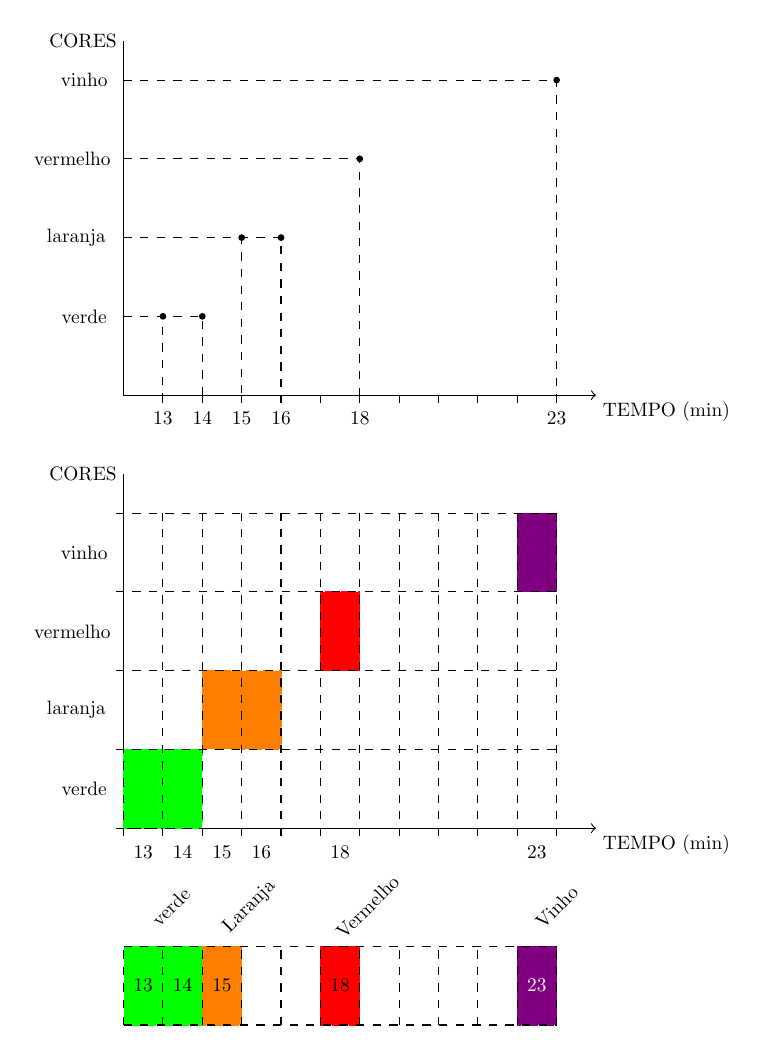
\begin{tikzpicture}
\draw[->](0,4.5) node[left, scale=.7]{CORES}--(0,0)--(6,0) node[below right, scale=.7]{TEMPO (min)};
\foreach \x in{1, 2, 3, 4, 5, 6, 7, 8, 9, 10, 11}
\draw(.5*\x, -.1)--(.5*\x,0);
\draw(.5,-.3) node[scale=.7]{13};
\draw(1,-.3) node[scale=.7]{14};
\draw(1.5,-.3) node[scale=.7]{15};
\draw(2,-.3) node[scale=.7]{16};
\draw(3,-.3) node[scale=.7]{18};
\draw(5.5,-.3) node[scale=.7]{23};
\draw(-.5,1)node[scale=.7]{verde};
\draw(-.6,2)node[scale=.7]{laranja};
\draw(-.65,3)node[scale=.7]{vermelho};
\draw(-.5,4)node[scale=.7]{vinho};
\draw[dashed](0,1)--(.5,1)--(.5,0);
\draw[dashed](0,1)--(1,1)--(1,0);
\draw[dashed](0,2)--(1.5,2)--(1.5,0);
\draw[dashed](0,2)--(2,2)--(2,0);
\draw[dashed](0,3)--(3,3)--(3,0);
\draw[dashed](0,4)--(5.5,4)--(5.5,0);
\draw[fill](.5,1)circle(1pt);
\draw[fill](1,1)circle(1pt);
\draw[fill](1.5,2)circle(1pt);
\draw[fill](2,2)circle(1pt);
\draw[fill](3,3)circle(1pt);
\draw[fill](5.5,4)circle(1pt);
\begin{scope}[yshift=-5.5cm]
\draw[->](0,4.5) node[left, scale=.7]{CORES}--(0,0)--(6,0) node[below right, scale=.7]{TEMPO (min)};
\foreach \x in{1, 2, 3, 4, 5, 6, 7, 8, 9, 10, 11}
\draw(.5*\x, -.1)--(.5*\x,0);
\draw(.25,-.3) node[scale=.7]{13};
\draw(.75,-.3) node[scale=.7]{14};
\draw(1.25,-.3) node[scale=.7]{15};
\draw(1.75,-.3) node[scale=.7]{16};
\draw(2.75,-.3) node[scale=.7]{18};
\draw(5.25,-.3) node[scale=.7]{23};
\draw(-.5,0.5)node[scale=.7]{verde};
\draw(-.6,1.5)node[scale=.7]{laranja};
\draw(-.65,2.5)node[scale=.7]{vermelho};
\draw(-.5,3.5)node[scale=.7]{vinho};
\draw[dashed,fill, color=green](0,0) rectangle (.5,1);
\draw[black,dashed,fill, color=green](.5,0) rectangle (1,1);
\draw[dashed,fill, color=orange](1,1) rectangle (1.5,2);
\draw[black,dashed,fill, color=orange](1.5,1) rectangle (2,2);
\draw[black,dashed,fill, color=red](2.5,2) rectangle (3,3);
\draw[black,dashed,fill, color=violet](5,3) rectangle (5.5,4);
\draw [color=black,dashed, xstep=.5cm,ystep=1cm] (-.1,-.1) grid (5.5,4);
\begin{scope}[yshift=-2.5cm]
\draw[dashed,fill, color=green](0,0) rectangle (1,1);
\draw[dashed,fill, color=orange](1,0) rectangle (1.5,1);
\draw[dashed,fill, color=red](2.5,0) rectangle (3,1);
\draw[black,dashed,fill, color=violet](5,0) rectangle (5.5,1);
\draw (.6,1.5)node[scale=.7, rotate=45]  {verde};
\draw (.25,.5)node[scale=.7]  {13};
\draw (.75,.5)node[scale=.7]  {14};
\draw(1.25,.5) node[scale=.7]{15};
\draw(2.75,.5) node[scale=.7]{18};
\draw[white](5.25,.5) node[scale=.7]{23};
\draw (1.6,1.5)node[scale=.7, rotate=45]  {Laranja};
\draw (3.1,1.5)node[scale=.7, rotate=45]  {Vermelho};
\draw (5.5,1.5)node[scale=.7, rotate=45]  {Vinho};
\draw [color=black,dashed, xstep=.5cm,ystep=1cm] (0,0) grid (5.5,1);
\end{scope}\end{scope}
\end{tikzpicture}

\item Uma possibilidade de reposta é: verde para $t\in [0,15[$, laranjar para $t\in[15,18[$, vermelho para $t\in[18,23[$ e vinho para $t\in[25,25]$

\item Ver item (b)

\end{enumerate}
\end{solucao}
\fi

\end{document}